\documentclass[sigconf]{webmedia}
% Para uma submissão double-blind real ao WebMedia, use:
% \documentclass[sigconf,anonymous,review]{webmedia}
% O exemplo do Overleaf historicamente mostrou o pacote lmodern, mas
% a própria documentação do template recomenda manter a família Libertine
% padrão do webmedia/acmart. Por isso, não há troca de fonte aqui.

\usepackage[utf8]{inputenc}
\usepackage[T1]{fontenc}
\usepackage[brazilian]{babel}
\usepackage{tabularx}

\urlstyle{tt}
\Urlmuskip=0mu plus 2mu\relax
\emergencystretch=1em

\AtBeginDocument{%
  \providecommand\BibTeX{{%
    \normalfont B\kern-0.5em{\scshape i\kern-0.25em b}\kern-0.8em\TeX}}}

\settopmatter{printacmref=true, printfolios=false}
\setevent{webmedia}
\proceedingsDetails[WebMedia'2025]{Proceedings of the Brazilian Symposium on Multimedia and the Web}{2025}{Rio de Janeiro, Brazil}
\ISSN{2966-2753}

\begin{document}

\title[Análise de Grafos em Embeddings do Reddit]{Análise de Grafos em uma Rede de Similaridade entre Subreddits Construída a partir de Embeddings do Reddit}

\author{Aluno Guilherme Neves}
\email{224116475}
\affiliation{%
  \institution{Universidade Federal da Bahia}
  \city{Salvador}
  \state{Bahia}
  \country{Brazil}
}
\renewcommand{\shortauthors}{Aluno Guilherme Neves}

\begin{abstract}
O dataset SNAP \textit{web-RedditEmbeddings} é analisado como uma rede de
similaridade semântica entre comunidades do Reddit. Como os dados
originais contêm embeddings e não uma lista explícita de arestas, o
grafo é construído por vizinhos mais próximos com similaridade de
cosseno sobre todos os 51.278 vetores de subreddits. O grafo simples,
não direcionado e ponderado resultante tem 51.278 vértices, 446.502 arestas,
densidade 0,000340, comprimento médio dos caminhos
$5,7044 \pm 0,1980$ com IC 95\%, clusterização média 0,2272 e 531.941
triângulos. A análise cobre métricas estruturais, algoritmos clássicos,
complexidade teórica e observada, intervalos de confiança dos tempos,
propriedade small-world, diagnóstico de lei de potência, robustez a
remoção aleatória e ataque direcionado, descoberta principal, comparação
com modelos clássicos, apêndices e instruções de reprodução. Os
resultados indicam uma rede esparsa, com componente gigante, forte
agrupamento local, caminhos curtos, cauda pesada de graus, tolerância a
falhas aleatórias e maior sensibilidade à remoção de hubs.
\end{abstract}

\begin{CCSXML}
<ccs2012>
   <concept>
       <concept_id>10002950.10003624.10003625</concept_id>
       <concept_desc>Mathematics of computing~Graph algorithms</concept_desc>
       <concept_significance>500</concept_significance>
   </concept>
   <concept>
       <concept_id>10003752.10010061.10010063</concept_id>
       <concept_desc>Theory of computation~Network flows</concept_desc>
       <concept_significance>300</concept_significance>
   </concept>
</ccs2012>
\end{CCSXML}

\ccsdesc[500]{Mathematics of computing~Graph algorithms}
\ccsdesc[300]{Theory of computation~Network flows}

\keywords{redes complexas, algoritmos de grafos, Reddit, embeddings, robustez, redes de pequeno mundo}

\maketitle

\section{Introdução}

O estudo aplica conceitos de Teoria dos Grafos e Redes Complexas a
um grafo real: tratamento de dados, análise estrutural, execução de
algoritmos clássicos, small-world, lei de potência, robustez e
comparação com modelos clássicos. O grafo é derivado do dataset
\textit{web-RedditEmbeddings}, publicado pelo SNAP~\cite{snapredditembeddings}.
O conjunto de dados representa usuários e subreddits por embeddings
temporais extraídos de interações em comunidades online
\cite{kumar2019predicting,kumar2018community}. Como o arquivo original
contém vetores e não uma lista explícita de arestas, a primeira etapa
metodológica foi construir uma rede de similaridade entre comunidades.

Todos os valores numéricos apresentados no artigo foram extraídos dos
artefatos do projeto na pasta \texttt{results}, incluindo JSON de
análise, CSVs de benchmarks e distribuição de graus. O código, os dados
tratados,
os resultados e as instruções de execução estão disponíveis no
repositório:
\url{https://github.com/guneves/TrabalhoGrafos}.

\subsection*{Resumo dos Resultados e Artefatos}

A Tabela~\ref{tab:mapa-correcao} resume os blocos principais da análise,
os pontos do texto onde cada resultado aparece e os artefatos do projeto
que permitem conferir os valores. A coluna ``Observação'' explícita
quando houve estimativa por amostragem, execução em subgrafo ou
conclusão conservadora.

\begin{table*}
  \caption{Resumo de leitura: resultados, localização no texto e artefatos conferíveis.}
  \label{tab:mapa-correcao}
  \small
  \begin{tabular}{@{}p{0.20\textwidth}p{0.24\textwidth}p{0.28\textwidth}p{0.18\textwidth}@{}}
    \toprule
    Bloco & Onde conferir & Artefato conferível & Observação \\
    \midrule
    Determinação do grafo & Seção 2 & \texttt{README.md}; \texttt{analysis\_results.json} & cálculo da matrícula até G110 \\
    Tratamento dos dados & Seção 3; Tabela~\ref{tab:tratamento} & \texttt{scripts/build\_graph.py}; \texttt{graph\_metadata.json} & embeddings convertidos em grafo simples kNN \\
    Análise estrutural & Seção 5; Tabela~\ref{tab:estrutural} & \texttt{analysis\_results.json}; \texttt{degree\_distribution.csv} & medidas estruturais completas \\
    Visualização & Figura~\ref{fig:grafo} & \texttt{graph\_visualization.png} em \texttt{LaTeX/results} & versão reduzida para legibilidade \\
    Algoritmos & Seção 6; Tabelas~\ref{tab:objetivo-algoritmos} e~\ref{tab:algoritmos} & \texttt{scripts/analyze\_graph.py}; \texttt{benchmark\_raw\_times.csv} & 30 execuções com média, desvio e IC 95\% \\
    Small-world & Seção 7; Apêndice A & \texttt{analysis\_results.json} & implementado no código do projeto \\
    Lei de potência & Seção 8; Apêndice B & \texttt{degree\_log\_pk.png}; \texttt{degree\_model\_comparison.png} & evidência sugestiva, não conclusão absoluta \\
    Robustez & Seção 9; Apêndice C & \texttt{robustness\_runs.csv}; \texttt{robustness.png} & 30 repetições aleatórias e ataque por grau \\
    Discussão e conclusão & Seções 10--12 & texto do relatório & descoberta, modelos clássicos e limitações \\
    Reprodução e checklist & Apêndices D--F & \texttt{README.md}; scripts do repositório & comandos de execução e checklist final \\
    \bottomrule
  \end{tabular}
\end{table*}

\section{Grafo Original e Determinação}

O dataset oficial é \textit{web-RedditEmbeddings}, da categoria
\textit{Online communities}, com tipo \textit{Reddit Embeddings}. A
página do SNAP informa 118.381 usuários, 51.278 subreddits, embeddings
de 300 dimensões e dados extraídos de janeiro de 2014 a abril de 2017.
A fonte oficial é
\url{https://snap.stanford.edu/data/web-RedditEmbeddings.html}. Os
arquivos brutos preservados localmente são:

\begin{verbatim}
data/raw/web-redditEmbeddings-subreddits.csv
data/raw/web-redditEmbeddings-users.csv
\end{verbatim}

A matrícula utilizada é 224116475. A regra usada para determinar o grafo
é
\[
\begin{aligned}
f(M) &= ((\text{soma dos dígitos}(M)) \times \\
     &\quad (\text{últimos dois dígitos}(M)+1)) \bmod 129.
\end{aligned}
\]
O cálculo passo a passo foi:

\begin{enumerate}
  \item Matrícula usada: 224116475.
  \item Soma dos dígitos: 32.
  \item Últimos dois dígitos: 75.
  \item Últimos dois dígitos + 1: 76.
  \item Multiplicação: $32 \times 76 = 2432$.
  \item Resultado do módulo 129: $2432 \bmod 129 = 110$.
  \item Grafo final escolhido: G110.
\end{enumerate}

Assim, a matrícula determina a posição do grafo em uma lista de 129
possibilidades. Nesta análise, o grafo G110 corresponde ao dataset
\textit{web-RedditEmbeddings}.

\section{Tratamento dos Dados}

O SNAP disponibiliza embeddings, não uma lista pronta de arestas. Por
isso, o tratamento necessário foi transformar vetores em uma rede de
similaridade entre comunidades. A versão analisada é uma rede simples,
não direcionada e ponderada de similaridade entre comunidades do Reddit.
Cada vértice representa um subreddit; duas comunidades são conectadas
quando uma aparece entre os vizinhos semanticamente mais próximos da
outra. Para métricas estruturais clássicas, o grafo foi considerado sem
peso; para algoritmos de caminho ponderado e MST, foi usado
$1-\mathrm{similaridade}$.

\begin{table*}
  \caption{Tratamento aplicado aos dados originais.}
  \label{tab:tratamento}
  \begin{tabular}{@{}p{0.13\textwidth}p{0.18\textwidth}p{0.13\textwidth}p{0.13\textwidth}p{0.19\textwidth}p{0.14\textwidth}@{}}
    \toprule
    Etapa & Tratamento aplicado & Antes & Depois & Justificativa & Impacto \\
    \midrule
    Fonte bruta & Download e preservação dos CSVs oficiais & 2 arquivos remotos & 2 arquivos em \texttt{data/raw} & garantir reprodutibilidade & não altera métricas \\
    Escolha de vértices & Subreddits como vértices & 118.381 usuários e 51.278 subreddits & 51.278 subreddits candidatos & foco em comunidades online & usuários não entram como vértices \\
    Uso de vértices & Todos os subreddits do CSV oficial & 51.278 candidatos & 51.278 vértices & usar todos os vértices disponíveis & elimina amostragem de vértices \\
    Normalização & vetores com norma 1 & embeddings de 300 dimensões & embeddings normalizados & calcular similaridade de cosseno por produto interno & prepara arestas \\
    Construção de arestas & kNN por similaridade de cosseno & sem arestas explícitas & 446.502 arestas & transformar embeddings em grafo analisável & define topologia \\
    Simplificação & união de pares kNN em grafo simples & vizinhanças direcionais possíveis & grafo simples não direcionado & métricas exigidas assumem grafo simples & remove duplicidade de pares \\
    Auto-loops & exclusão do próprio vértice no kNN & similaridade de cada vértice consigo mesmo & zero auto-loops & auto-loops não ajudam nas métricas exigidas & evita inflar graus e triângulos \\
    Pesos & $1-\mathrm{similaridade}$ & similaridade de cosseno & pesos não negativos & menor peso indica maior semelhança & permite Dijkstra/MST \\
    Componentes & verificação de conectividade & grafo tratado & 3 componentes; maior com 51.245 vértices & identificar a estrutura conexa usada nos caminhos & caminhos por amostragem de fontes \\
    \bottomrule
  \end{tabular}
\end{table*}

Os dados tratados usados nas análises estão em
\texttt{nodes.csv}, \texttt{edges.csv} e
\texttt{graph\_metadata.json}, na pasta \texttt{data/processed}. O README do repositório
descreve como reproduzir o pipeline completo.

\section{Metodologia}

As métricas estruturais foram calculadas sobre a versão não ponderada
quando a definição clássica depende do número de arestas. Dijkstra,
Bellman-Ford, Floyd-Warshall e Kruskal usaram pesos. Diâmetro, raio e
comprimento médio dos caminhos foram estimados por 16 fontes na maior
componente por causa do tamanho do grafo; nessa situação, diâmetro e
raio são valores observados na amostra, e o comprimento médio tem IC
95\% de $\pm 0,1980$. Cada algoritmo foi executado 30 vezes. Os
intervalos de confiança de 95\% usam Normal/Z quando $n \geq 30$ e
t-Student quando $n < 30$; nesta execução, os benchmarks usaram
Normal/Z. Os tempos individuais de cada repetição foram
exportados em \texttt{benchmark\_raw\_times.csv}, enquanto
\texttt{benchmark\_times.csv} contém média, desvio padrão e IC 95\%;
ambos ficam na pasta \texttt{results}.

Para evitar ambiguidade na correção, sempre que uma medida foi estimada
ou restringida por custo computacional o texto informa a política usada.
Assim, diâmetro e raio são apresentados como limites observados por
amostragem, Bellman-Ford e Floyd-Warshall são marcados como execuções em
subgrafos, e a lei de potência é tratada como evidência sugestiva, não
como afirmação estatística definitiva.

As rotinas de grafo usadas na análise foram implementadas no
próprio projeto em Python, sem bibliotecas prontas como NetworkX ou
igraph. As dependências externas, como \texttt{numpy}, \texttt{pandas}
e \texttt{Pillow}, foram usadas para vetorização, leitura de CSV e
figuras, não para calcular
small-world, robustez, Tarjan, Kruskal ou os percorrimentos.

\section{Análise Estrutural}

\begin{table*}
  \caption{Métricas estruturais do grafo tratado.}
  \label{tab:estrutural}
  \begin{tabular}{@{}p{0.21\textwidth}p{0.13\textwidth}p{0.10\textwidth}p{0.34\textwidth}p{0.12\textwidth}@{}}
    \toprule
    Medida & Valor & Computada? & Interpretação & Justificativa \\
    \midrule
    Número de vértices & 51.278 & Sim & quantidade de subreddits usados do arquivo oficial & N/A \\
    Número de arestas & 446.502 & Sim & pares de comunidades semanticamente próximas & N/A \\
    Grau mínimo & 10 & Sim & efeito esperado do kNN com $k=10$ & N/A \\
    Grau máximo & 273 & Sim & existe ao menos um hub semântico muito conectado & N/A \\
    Grau médio & 17,4150 & Sim & rede esparsa, mas com conexões suficientes para formar uma componente gigante & N/A \\
    Distribuição de graus & CSV gerado & Sim & cauda pesada e hubs aparecem na frequência dos graus & N/A \\
    Densidade & 0,000340 & Sim & apenas pequena fração dos pares possíveis está conectada & N/A \\
    Componentes conexas & 3 & Sim & há uma componente gigante e duas pequenas & N/A \\
    Tamanho das componentes & 51.245, 18, 15 & Sim & a maior componente concentra quase todos os vértices, mas o grafo não é totalmente conectado & N/A \\
    Diâmetro & 13 & Sim & limite inferior observado por amostragem no modo sampled & N/A \\
    Raio & 10 & Sim & limite superior observado por amostragem no modo sampled & N/A \\
    Comprimento médio & $5,7044 \pm 0,1980$ & Sim & poucos intermediários separam comunidades & N/A \\
    Clusterização média & 0,2272 & Sim & há forte agrupamento local & N/A \\
    Número de triângulos & 531.941 & Sim & muitas triplas de subreddits semanticamente próximos & N/A \\
    Visualização & grafo reduzido & Sim & amostra visual para evitar sobreposição excessiva & N/A \\
    \bottomrule
  \end{tabular}
\end{table*}

A Figura~\ref{fig:grafo} mostra uma amostra reduzida de 420 vértices,
escolhida para tornar a estrutura legível. Os vértices azuis destacam
hubs por grau e os verdes mostram vizinhos amostrados; as arestas
representam relações kNN por similaridade. O bloco principal denso
indica a componente gigante, enquanto o agrupamento separado evidencia
que existem componentes pequenas. A figura não substitui as métricas
completas, mas ajuda a ver a coexistência de alta conectividade local e
hubs.

Portanto, as medidas estruturais principais foram computadas e estão
presentes na Tabela~\ref{tab:estrutural}. As ressalvas são
metodológicas: diâmetro, raio e caminho médio foram obtidos por
amostragem de fontes na maior componente conexa devido ao tamanho da
rede, e a própria tabela informa essa condição para evitar interpretação
como cálculo exato de todos os pares.

\begin{figure*}
  \centering
  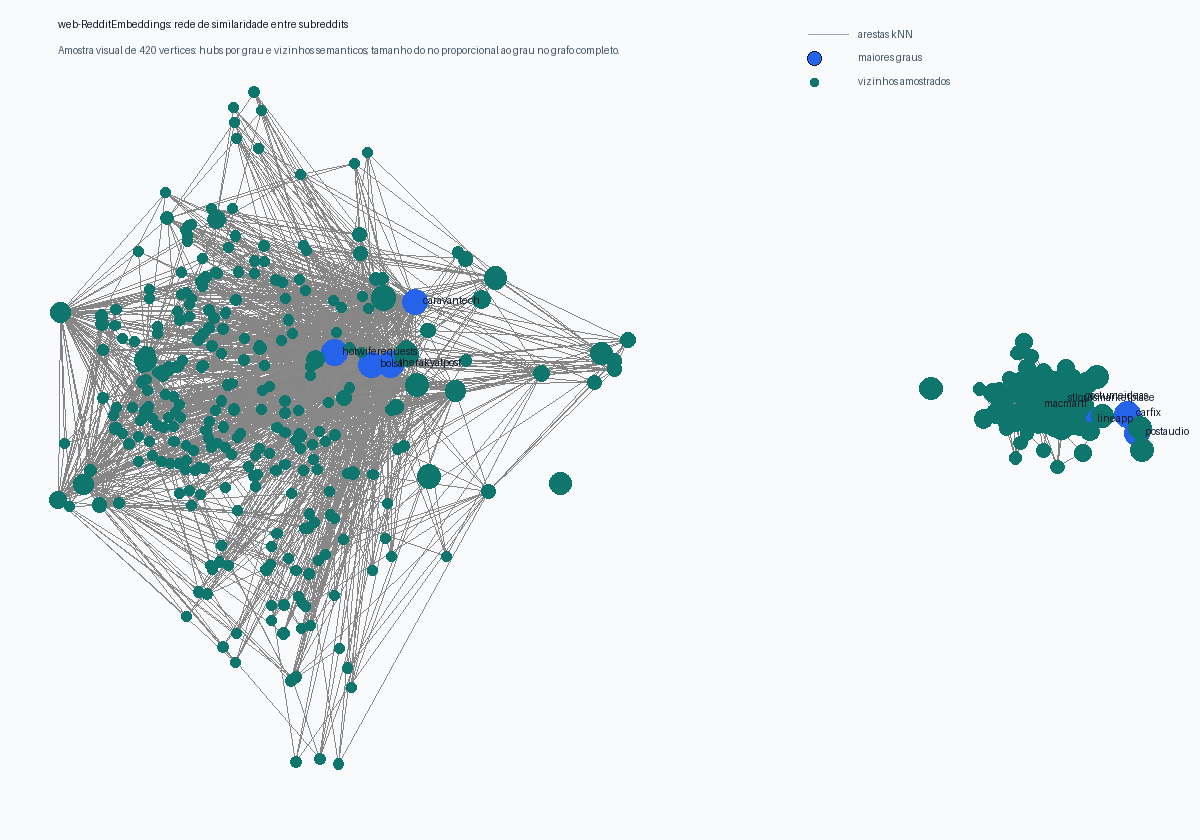
\includegraphics[width=\textwidth]{results/graph_visualization.png}
  \caption{Amostra visual da rede de similaridade entre subreddits.}
  \Description{Grafo amostrado com bloco principal denso, agrupamento menor separado, hubs destacados em azul e demais vértices em verde.}
  \label{fig:grafo}
\end{figure*}

A Figura~\ref{fig:histgraus} apresenta o histograma de graus. O eixo
vertical está em escala log10 de frequência. A maior concentração está
nos graus baixos, especialmente perto do grau mínimo 10 imposto pelo
kNN, e as barras diminuem rapidamente conforme o grau aumenta. A
presença de poucos vértices até grau 273 indica uma cauda longa e a
existência de subreddits semanticamente parecidos com muitos outros.

\begin{figure}
  \centering
  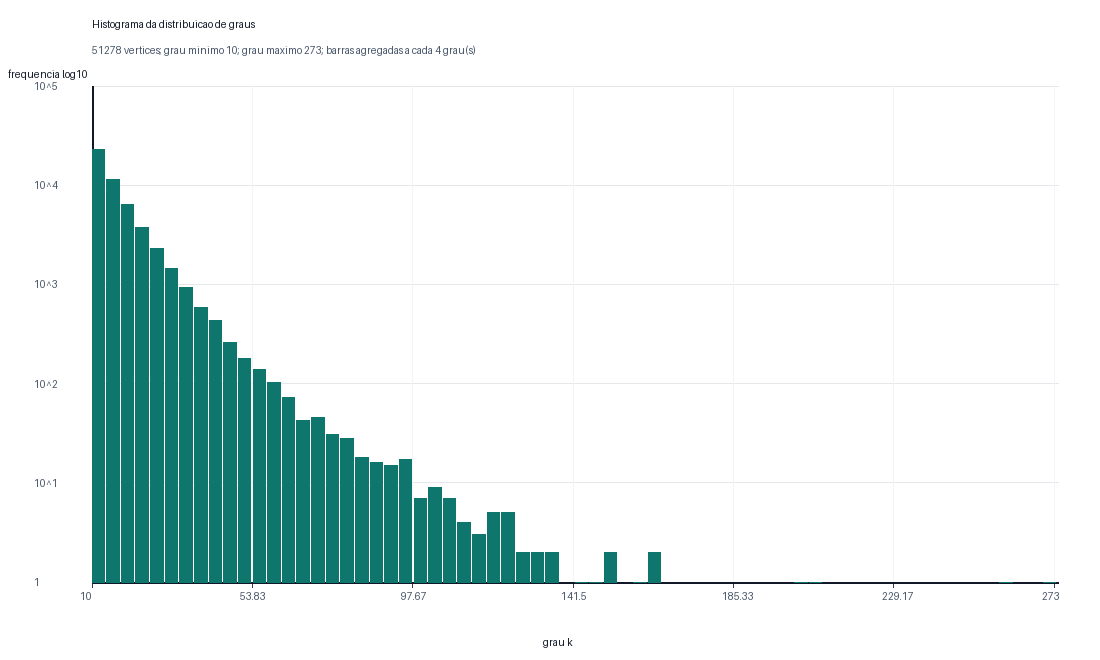
\includegraphics[width=\linewidth]{results/degree_histogram.png}
  \caption{Histograma da distribuição de graus em escala logarítmica.}
  \Description{Barras decrescentes indicam muitos vértices com grau baixo ou moderado e poucos hubs de grau elevado.}
  \label{fig:histgraus}
\end{figure}

A Figura~\ref{fig:ccdf} mostra a CCDF dos graus: para cada grau $k$, ela
indica a fração de vértices com grau maior ou igual a $k$. Em escala
log-log, a porção central fica aproximadamente linear, sustentando a
hipótese de cauda pesada. As curvaturas nas extremidades mostram que o
gráfico deve ser lido como evidência visual, não como prova estatística
isolada de lei de potência. O arquivo
\texttt{degree\_distribution.svg}, na pasta \texttt{results}, contém a mesma visualização,
mantida como alias do gráfico de distribuição acumulada.

\begin{figure}
  \centering
  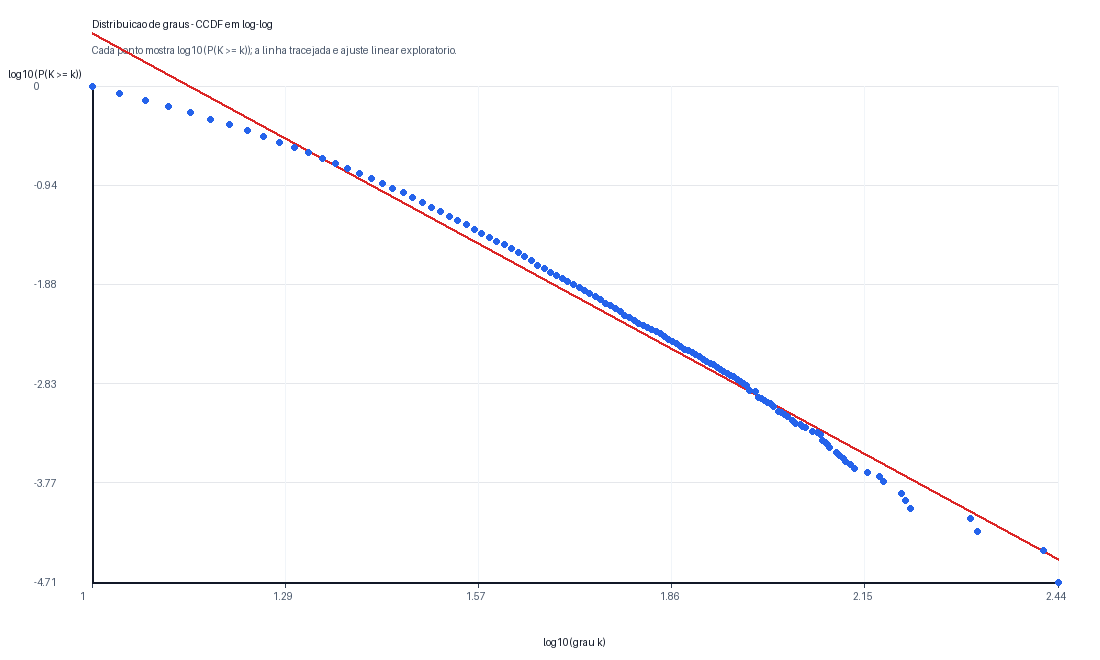
\includegraphics[width=\linewidth]{results/degree_ccdf.png}
  \caption{CCDF da distribuição de graus em log-log.}
  \Description{Pontos decrescentes em log-log com uma reta de ajuste exploratório sobre a porção central.}
  \label{fig:ccdf}
\end{figure}

\section{Algoritmos Implementados}

\begin{table*}
  \caption{Objetivo, funcionamento e complexidade teórica dos algoritmos.}
  \label{tab:objetivo-algoritmos}
  \begin{tabular}{@{}p{0.16\textwidth}p{0.62\textwidth}p{0.15\textwidth}@{}}
    \toprule
    Algoritmo & Objetivo, funcionamento e condições & Complexidade \\
    \midrule
    BFS & visita a origem, depois seus vizinhos, depois os vizinhos dos vizinhos; aplicável para medir alcançabilidade em grafos ponderados ou não quando o peso não importa & $O(V+E)$ \\
    DFS & explora um ramo até o fim antes de retroceder; aplicável para percorrimento e base de análises de conectividade & $O(V+E)$ \\
    Eulerianidade & checa se o grafo não direcionado é conectado e se todos os graus são pares & $O(V+E)$ \\
    Dijkstra & relaxa arestas em ordem de distância mínima por fila de prioridade; aplicável porque $1-\mathrm{similaridade}$ não é negativo & $O((V+E)\log V)$ \\
    Bellman-Ford & relaxa todas as arestas repetidamente e tolera pesos negativos; aqui é aplicável, mas redundante, pois não há pesos negativos & $O(VE)$ \\
    Floyd-Warshall & atualiza uma matriz de distâncias considerando cada vértice como intermediário; aplicável conceitualmente, mas caro no grafo completo & $O(V^3)$ \\
    Tarjan & usa tempos de descoberta e valores low-link para identificar pontos de articulação e pontes na versão não direcionada & $O(V+E)$ \\
    Kruskal/MST & ordena arestas por peso e une componentes com union-find; se o grafo for desconexo, o resultado é uma floresta geradora mínima & $O(E\log E)$ \\
    \bottomrule
  \end{tabular}
\end{table*}

\begin{table*}
  \caption{Tempos observados dos algoritmos com média, desvio padrão e IC 95\%.}
  \label{tab:algoritmos}
  \small
  \begin{tabular}{@{}p{0.16\textwidth}p{0.10\textwidth}p{0.17\textwidth}p{0.11\textwidth}p{0.10\textwidth}p{0.12\textwidth}p{0.12\textwidth}@{}}
    \toprule
    Algoritmo & Aplicável? & Complexidade & Tempo médio (s) & Desvio padrão (s) & IC 95\% (s) & Resultado \\
    \midrule
    BFS & Sim & $O(V+E)$ & 0,093890 & 0,008430 & $\pm 0,003017$ & 51.245 \\
    DFS & Sim & $O(V+E)$ & 0,200372 & 0,010345 & $\pm 0,003702$ & 51.245 \\
    Eulerianidade & Sim & $O(V+E)$ & 0,000000 & 0,000000 & $\pm 0,000000$ & False \\
    Dijkstra & Sim & $O((V+E)\log V)$ & 0,177694 & 0,006897 & $\pm 0,002468$ & 51.245 \\
    Bellman-Ford & subgrafo & $O(VE)$ & 0,000005 & 0,000002 & $\pm 0,000001$ & 1 \\
    Floyd-Warshall & subgrafo & $O(V^3)$ & 0,000256 & 0,000014 & $\pm 0,000005$ & 70 \\
    Tarjan & Sim & $O(V+E)$ & 0,250317 & 0,044932 & $\pm 0,016079$ & 5; 1 \\
    Kruskal/MST & Sim & $O(E\log E)$ & 0,327248 & 0,012688 & $\pm 0,004540$ & 51.275 \\
    \bottomrule
  \end{tabular}
\end{table*}

A Figura~\ref{fig:tempos} usa eixo Y em log10 de segundos; por isso,
diferencas pequenas na altura das barras representam ordens de grandeza.
As barras mostram a média das 30 execuções e as hastes mostram o IC
95\%. A verificação de eulerianidade é muito rápida, Bellman-Ford e
Floyd-Warshall ficam pequenos porque foram executados em subgrafos,
enquanto Tarjan e Kruskal aparecem entre os mais custosos por percorrerem
a estrutura grande do grafo.

\begin{figure}
  \centering
  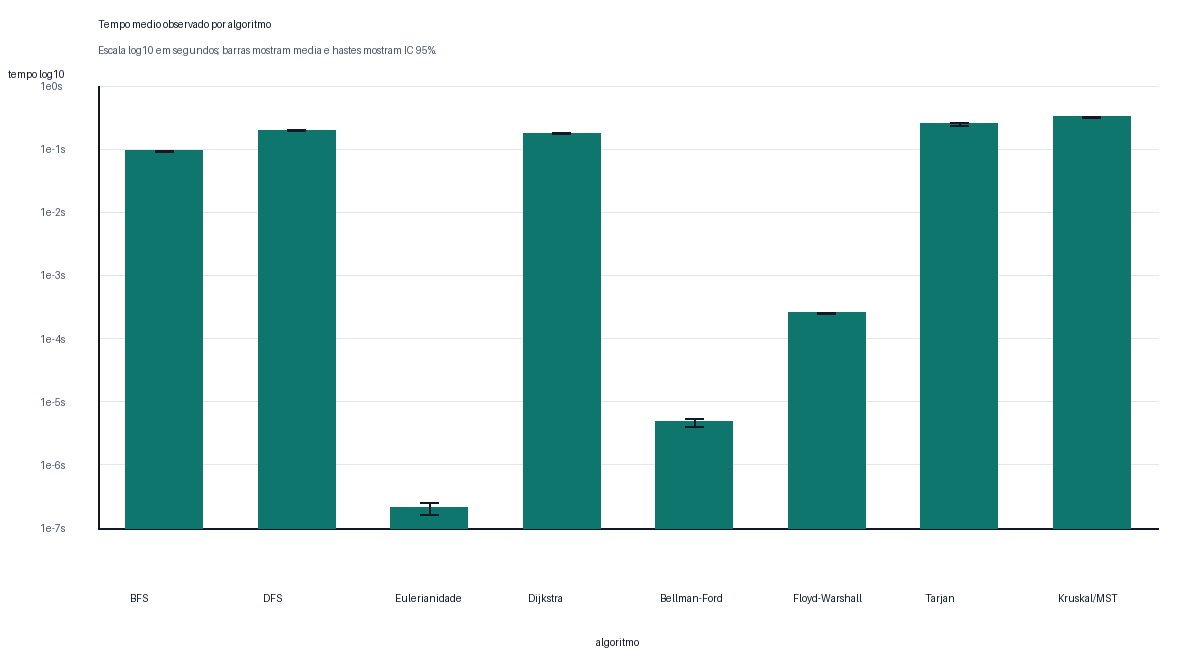
\includegraphics[width=\linewidth]{results/algorithm_times.png}
  \caption{Tempos médios observados por algoritmo, com IC 95\%.}
  \Description{Gráfico de barras em escala logarítmica comparando tempos médios de BFS, DFS, Dijkstra, Tarjan, Kruskal e algoritmos em subgrafos.}
  \label{fig:tempos}
\end{figure}

BFS alcançou 51.245 vértices e DFS alcançou 51.245, isto é, a componente
da origem usada nos testes. O grafo não é euleriano, pois nem todos os
vértices têm grau par. Dijkstra alcançou 51.245 vértices com pesos não
negativos. Bellman-Ford foi executado em subgrafo de 120 vértices e
Floyd-Warshall em subgrafo de 70 vértices, com justificativa técnica de
custo. Tarjan encontrou 5 pontos de articulação e 1 ponte. Kruskal gerou
uma floresta geradora mínima com 51.275 arestas e peso total 3127,7570.

\section{Análise de Small-World}

A análise verifica se o grafo apresenta indícios de propriedade small-world, se essa
interpretação faz sentido para a rede e qual é sua implicação prática.

\begin{table}
  \caption{Comparação small-world com grafos aleatórios equivalentes.}
  \label{tab:small-world}
  \small
  \setlength{\tabcolsep}{3pt}
  \begin{tabularx}{\linewidth}{@{}p{0.27\linewidth}p{0.16\linewidth}p{0.25\linewidth}X@{}}
    \toprule
    Métrica & Grafo real & Aleatórios & Comparação \\
    \midrule
    Comprimento médio & 5,7044 & $4,0575 \pm 0,0314$ & mesma ordem \\
    Clusterização média & 0,2272 & $0,0003 \pm 0,0000$ & real 661,63 vezes maior \\
    \bottomrule
  \end{tabularx}
\end{table}

Há indícios relevantes, de moderados a fortes, de small-world no sentido
clássico de Watts e Strogatz~\cite{watts1998collective}. O
comprimento médio dos caminhos permanece pequeno em termos práticos e da
mesma ordem do aleatório, embora seja maior que o do grafo aleatório
equivalente; ao mesmo tempo, a clusterização real é muito maior. Isso faz
sentido para subreddits, pois comunidades temáticas formam grupos locais
densos, mas ainda se conectam por caminhos curtos via interesses
intermediários. A implicação prática é comunicação ou propagação
eficiente entre comunidades com forte agrupamento local. O cálculo foi
feito com BFS, contagem de triângulos/clusterização e grafos aleatórios
implementados no script \texttt{scripts/analyze\_graph.py}, evitando
bibliotecas prontas de análise de redes.

\section{Análise de Lei de Potência}

A distribuição de graus foi analisada para verificar se há indícios de
lei de potência. A
distribuição sugere cauda pesada e presença de hubs, mas não
permite afirmar rigorosamente uma lei de potência sem teste estatístico
completo, seguindo a cautela metodológica recomendada por
Clauset et al.~\cite{clauset2009powerlaw}. A CCDF em escala log-log teve inclinação estimada 3,4808 e
$R^2=0,9867$. Como melhoria, também foi aplicado um ajuste discreto
exploratório por máxima verossimilhança: $\alpha=4,6905$,
$x_{\min}=42$, cauda com 1.454 vértices (2,84\%) e KS = 0,0118. A
cauda ajustada favoreceu lei de potência sobre exponencial no diagnóstico
exploratório de log-verossimilhança.

\begin{table}
  \caption{Amostra da tabela de $P(k)$ usada no gráfico log-log.}
  \label{tab:pk}
  \begin{tabular}{@{}rrrrr@{}}
    \toprule
    $k$ & Freq. & $P(k)$ & $\log(k)$ & $\log(P(k))$ \\
    \midrule
    10 & 7753 & 0,151195 & 2,3026 & -1,8892 \\
    11 & 5972 & 0,116463 & 2,3979 & -2,1502 \\
    12 & 4818 & 0,093958 & 2,4849 & -2,3649 \\
    13 & 4240 & 0,082687 & 2,5649 & -2,4927 \\
    14 & 3580 & 0,069816 & 2,6391 & -2,6619 \\
    15 & 3041 & 0,059304 & 2,7081 & -2,8251 \\
    16 & 2654 & 0,051757 & 2,7726 & -2,9612 \\
    17 & 2269 & 0,044249 & 2,8332 & -3,1179 \\
    18 & 1976 & 0,038535 & 2,8904 & -3,2562 \\
    19 & 1687 & 0,032899 & 2,9444 & -3,4143 \\
    273 & 1 & 0,000020 & 5,6095 & -10,8450 \\
    \bottomrule
  \end{tabular}
\end{table}

A Figura~\ref{fig:logpk} usa a probabilidade pontual de cada grau, não a
probabilidade acumulada. A tendência decrescente quase linear reforça a
presença de cauda pesada, mas os pontos dos graus altos ficam ruidosos
porque há poucos vértices em cada grau extremo. Portanto, ela é útil como
evidência visual complementar a CCDF e ao ajuste MLE.

\begin{figure}
  \centering
  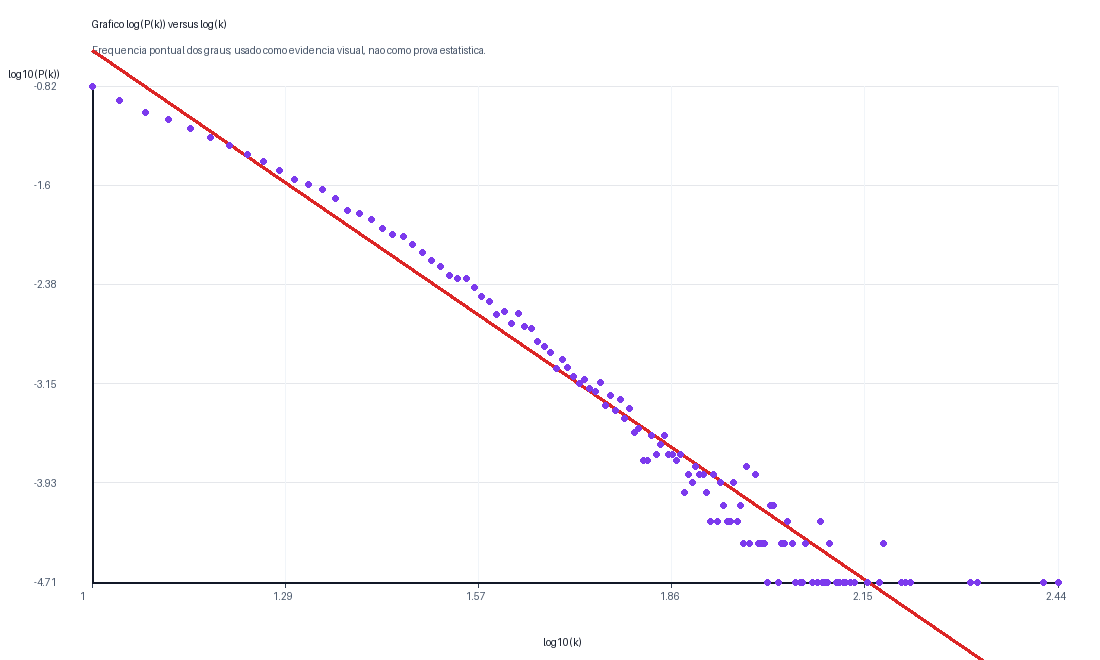
\includegraphics[width=\linewidth]{results/degree_log_pk.png}
  \caption{Gráfico de $\log(P(k))$ versus $\log(k)$.}
  \Description{Pontos em escala log-log com tendência decrescente e reta de ajuste exploratório.}
  \label{fig:logpk}
\end{figure}

A Figura~\ref{fig:modelosgrau} compara a distribuição observada com uma
Poisson de média igual ao grau médio e uma normal com a mesma média e
desvio padrão dos graus observados. Como o eixo Y está em log10,
probabilidades visualmente nulas usam um piso numérico apenas para
renderização. A curva observada mantém probabilidade visível por uma
faixa muito maior de graus do que Poisson e normal com média comparável.
As distribuições homogêneas concentram massa perto da média, enquanto o
grafo real preserva vértices raros de grau muito alto.

\begin{figure}
  \centering
  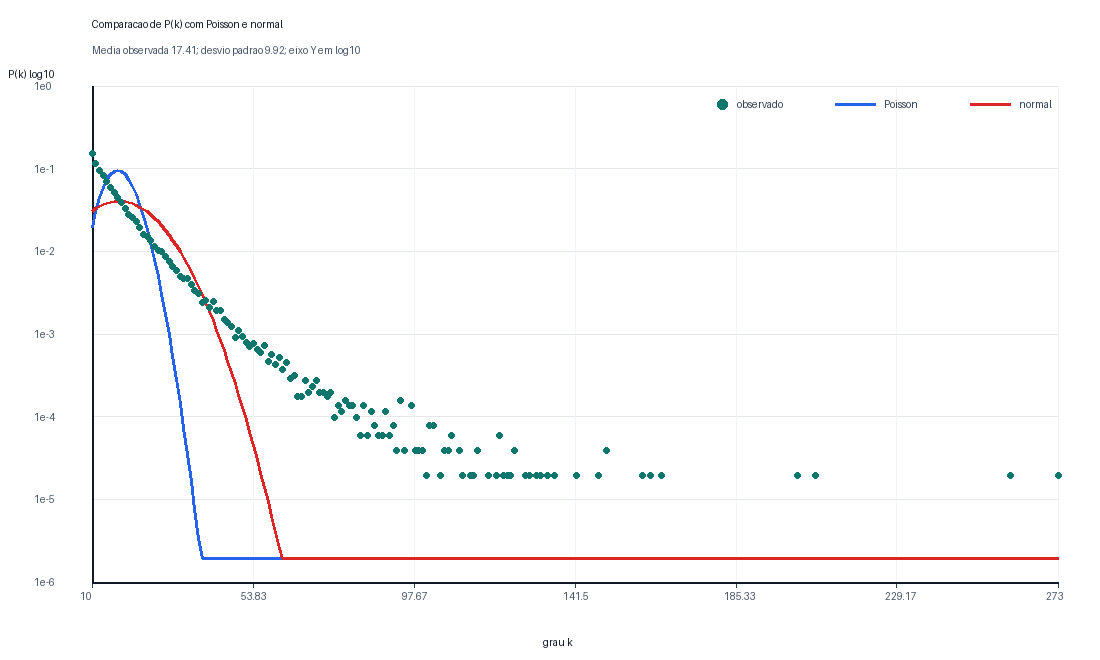
\includegraphics[width=\linewidth]{results/degree_model_comparison.png}
  \caption{Comparação de $P(k)$ observada com Poisson e normal.}
  \Description{Pontos observados formam uma cauda longa; curvas de Poisson e normal caem rapidamente perto da média.}
  \label{fig:modelosgrau}
\end{figure}

Portanto, há muitos vértices em graus baixos ou moderados, e poucos
vértices de grau muito alto, como o grau máximo 273, muito acima do grau
médio 17,4150. Há indícios compatíveis com lei de potência e rede
parcialmente livre de escala, mas a evidência é sugestiva, não
conclusiva.

\section{Análise de Robustez}

A robustez do grafo foi avaliada por remoção aleatória de 5\% dos vértices e pela
remoção dos 5\% mais centrais. Foram removidos 2.564
vértices, equivalentes a 5\% da rede tratada. A remoção aleatória foi
repetida 30 vezes; o ataque direcionado removeu os 5\% de maior grau.
Como a remoção pode fragmentar a rede, o comprimento médio dos caminhos
foi calculado na maior componente conexa remanescente e estimado por
amostragem de fontes.

\begin{table*}
  \caption{Robustez após remoção de 5\% dos vértices.}
  \label{tab:robustez}
  \small
  \setlength{\tabcolsep}{3pt}
  \begin{tabularx}{\textwidth}{@{}p{0.16\textwidth}p{0.10\textwidth}p{0.20\textwidth}p{0.18\textwidth}X@{}}
    \toprule
    Métrica & Original & Remoção aleatória 5\% & Remoção dos 5\% mais centrais & Interpretação \\
    \midrule
    Maior componente & 51.278 & $48680,6000 \pm 1,6482$ & 48.641 & ataque central reduz mais a componente principal \\
    Número de componentes & 3 & $3,1667 \pm 0,1356$ & 42 & ataque central fragmenta a rede \\
    Comprimento médio & 5,7044 & $5,9922 \pm 0,0706$ & 6,3694 & caminhos crescem mais no ataque central \\
    Fração de nós isolados & 0 & $0,0000 \pm 0,0000$ & 0,0008 & ataque central gera isolados \\
    \bottomrule
  \end{tabularx}
\end{table*}

A Figura~\ref{fig:robustez} resume os ensaios de robustez. As caixas
azuis mostram as 30 remoções aleatórias de 5\% dos vértices, enquanto o
ponto vermelho mostra o ataque por grau. A remoção aleatória quase não
muda a maior componente e mantém poucas componentes. O ataque direcionado
fica claramente pior no número de componentes, na fração isolada e no
comprimento médio, mostrando que os hubs são importantes para encurtar
caminhos e reduzir fragmentação.

\begin{figure*}
  \centering
  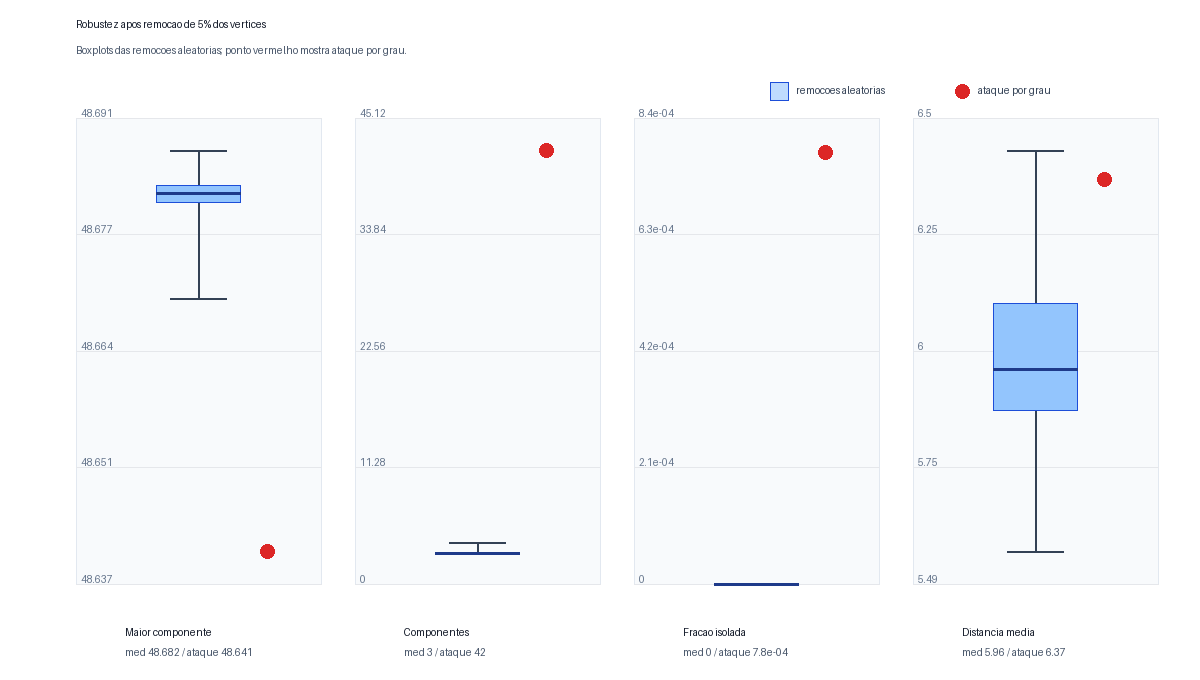
\includegraphics[width=\textwidth]{results/robustness.png}
  \caption{Boxplots de robustez para remoção aleatória e ataque por grau.}
  \Description{Quatro painéis com maior componente, componentes, fração isolada e distância média; caixas azuis indicam remoções aleatórias e pontos vermelhos indicam ataque por grau.}
  \label{fig:robustez}
\end{figure*}

O grafo é muito robusto a falhas aleatórias, pois a maior componente
reteve em média 99,93\% dos vértices restantes. A remoção dos 5\%
vértices de maior grau é mais danosa: fragmenta a rede em 42
componentes, gera nós isolados e aumenta o comprimento médio dos
caminhos. Portanto, há vulnerabilidade maior a ataques direcionados do
que a falhas aleatórias.

\clearpage

\section{Principal Constatação Empírica}

A principal constatação empírica é que a rede de subreddits é altamente
agrupada e, ao mesmo tempo, redundante. Esse padrão aparece no
clustering médio 0,2272, nos 531.941 triângulos e no resultado de
Tarjan: 5 pontos de articulação e 1 ponte. Em termos práticos,
comunidades semanticamente próximas não dependem de uma única rota:
mesmo quando hubs são removidos, a maior componente ainda retém 99,85\%
dos vértices restantes, embora o ataque tenha aumentado a fragmentação e
o caminho médio.

\section{Comparação com Modelos Clássicos}

O grafo foi comparado com os modelos clássicos Erdős-Rényi, Barabási-Albert e
Watts-Strogatz~\cite{erdos1959random,barabasi1999emergence,watts1998collective}.

\begin{table}[H]
  \caption{Comparação qualitativa com modelos clássicos.}
  \label{tab:modelos}
  \small
  \setlength{\tabcolsep}{3pt}
  \begin{tabularx}{\linewidth}{@{}p{0.22\linewidth}Xp{0.22\linewidth}@{}}
    \toprule
    Modelo & Evidências principais & Aproximação \\
    \midrule
    Erdős-Rényi & explica apenas esparsidade e componente gigante; falha em clusterização e grau máximo. & fraca \\
    Barabási-Albert & captura hubs, cauda pesada e maior vulnerabilidade a ataque central, mas não o alto agrupamento local. & parcial \\
    Watts-Strogatz & combina alto clustering e caminhos curtos, que são os sinais empíricos mais fortes da rede. & mais próximo \\
    \bottomrule
  \end{tabularx}
\end{table}

A aproximação mais forte é com Watts-Strogatz/small-world, com traços
parciais de Barabási-Albert por causa dos hubs. A aproximação com
Erdős-Rényi é fraca, porque a clusterização real é muito maior que a
esperada em um grafo aleatório homogêneo. Como as arestas foram
criadas por similaridade semântica entre embeddings, nenhum modelo
clássico descreve completamente o mecanismo de formação do grafo.

\clearpage

\section{Discussão Crítica}

O resultado depende da escolha de $k$. Como todos os subreddits
disponíveis são usados, não há amostragem de vértices; ainda assim, como
o dataset original é embedding, qualquer grafo derivado exige uma regra
metodológica de criação de arestas. Valores maiores de $k$ aumentariam
densidade e poderiam reduzir diâmetro; valores menores poderiam
fragmentar a rede.

Bellman-Ford e Floyd-Warshall foram executados em subgrafos por custo
computacional, portanto seus tempos medem a implementação e a
aplicabilidade conceitual, não o custo do grafo completo. A análise de
lei de potência combina diagnóstico visual e ajuste MLE discreto
exploratório, mas ainda não substitui um estudo estatístico completo com
bootstrap de p-valor e comparações formais adicionais.

\section{Conclusão}

A análise aplicou tratamento de dados, construção de grafo, análise
estrutural, algoritmos clássicos, small-world, lei de potência e robustez
ao dataset \textit{web-RedditEmbeddings}. A rede tratada é dominada por
uma componente gigante, pouco densa, altamente clusterizada, robusta a
falhas aleatórias e mais sensível à remoção de hubs semânticos. A
principal descoberta foi que a rede combina redundancia local, refletida
por 531.941 triângulos e clusterização 0,2272, com poucos pontos
estruturais realmente críticos: Tarjan encontrou 5 pontos de articulação
e 1 ponte.

\begin{acks}
A elaboracao do artigo utilizou os artefatos computacionais gerados no
repositório do projeto.
\end{acks}

\bibliographystyle{ACM-Reference-Format}
\bibliography{artigo_webmedia_referencias}

\clearpage

\appendix

\section{Small-World}

A definição operacional de pequeno mundo foi baseada nas leituras:
\url{https://en.wikipedia.org/wiki/Small-world_network} e
\url{https://pt.wikipedia.org/wiki/Redes_de_pequeno_mundo}. Uma rede
possui propriedade small-world quando a distância média entre vértices é
pequena e o coeficiente de clusterização é alto. Formalmente, a
comparação adotada na análise foi:
\[
  L(G) \approx L_{\text{aleatório}}
  \quad\text{e}\quad
  C(G) \gg C_{\text{aleatório}}.
\]
No grafo tratado, a conclusão aparece na Tabela~\ref{tab:small-world}: o
comprimento médio está na mesma ordem de grandeza do aleatório
equivalente, enquanto a clusterização é centenas de vezes maior.

\section{Lei de Potência}

A definição de lei de potência foi baseada em
\url{https://en.wikipedia.org/wiki/Power_law}. A hipótese investigada é
se a probabilidade de um vértice ter grau $k$ segue aproximadamente
\[
  P(k) \sim Ck^{-\gamma},
\]
com $\gamma > 1$. A intuição é que, em uma rede com lei de potência,
muitos vértices têm grau pequeno e poucos vértices funcionam como hubs
de grau muito alto. Para verificar isso, a rotina computacional calcula a
distribuição de graus, gera histograma, CCDF e o gráfico
$\log(P(k))$ versus $\log(k)$. A análise da Seção~8 também inclui um
ajuste exploratório por máxima verossimilhança e comparação visual com
Poisson e normal.

\section{Robustez}

O procedimento de robustez mediu o efeito da remoção de 5\% dos
vértices. Como o grafo original já tem 3 componentes, as
distâncias após remoção foram calculadas na maior componente conexa
remanescente. Foram medidas quatro grandezas: tamanho da maior
componente, número de componentes, distância média e fração de vértices
isolados.

Para a remoção aleatória, foram executadas 30 repetições, removendo
vértices uniformemente ao acaso e reportando média, desvio padrão e IC
95\%. Para o ataque direcionado, a centralidade escolhida foi grau,
porque remove diretamente os hubs da rede. O ranking é fixo: calcula-se
o grau no grafo original,
ordenam-se os vértices do maior para o menor grau, removem-se os 5\%
mais centrais e recalculam-se as mesmas métricas. A comparação aparece
na Seção~9.

\section{Código Principal}

O código completo está organizado em scripts reprodutíveis. O repositório
da entrega é \url{https://github.com/guneves/TrabalhoGrafos}. Os scripts
principais são:

\begin{itemize}
  \item \texttt{scripts/download\_data.py}: baixa os CSVs oficiais.
  \item \texttt{scripts/build\_graph.py}: lê embeddings, normaliza vetores, constrói kNN, salva vértices/arestas e visualização.
  \item \texttt{scripts/analyze\_graph.py}: calcula métricas, algoritmos, tempos, small-world com grafos aleatórios, lei de potência com MLE exploratório e robustez.
\end{itemize}

\section{Como Reproduzir}

Pipeline detalhado:

\begin{verbatim}
pip install -r requirements.txt
python scripts/download_data.py
python scripts/build_graph.py --k 10
python scripts/analyze_graph.py --benchmark-runs 30 \
  --robustness-runs 30 \
  --path-samples 16 \
  --random-graphs 5
\end{verbatim}

Atalho equivalente:

\begin{verbatim}
python main.py
\end{verbatim}

\clearpage

\begin{table*}
  \caption{Checklist final de cobertura da análise.}
  \label{tab:checklist}
  \begin{tabular}{@{}p{0.45\textwidth}p{0.12\textwidth}p{0.34\textwidth}@{}}
    \toprule
    Item & Atendido? & Onde aparece \\
    \midrule
    Calculo do grafo pela matrícula & Sim & Seção 2 \\
    Tratamento dos dados informado & Sim & Seção 3 \\
    Número de vértices e arestas & Sim & Seção 5 \\
    Grau mínimo, máximo e médio & Sim & Seção 5 \\
    Distribuição de graus & Sim & Seções 5 e 8; gráficos de graus \\
    Densidade & Sim & Seção 5 \\
    Componentes conexas e tamanhos & Sim & Seção 5 \\
    Diâmetro, raio e caminho médio & Sim & Seção 5 \\
    Clusterização média e triângulos & Sim & Seção 5 \\
    Visualização do grafo & Sim & Figura~\ref{fig:grafo} \\
    BFS, DFS, Eulerianidade, Dijkstra, Bellman-Ford, Floyd-Warshall, Tarjan e Kruskal & Sim & Seção 6 \\
    Complexidade teórica, tempo real, média, desvio padrão e IC & Sim & Seção 6 \\
    Small-world & Sim & Seção 7 \\
    Lei de potência & Sim & Seção 8 \\
    Robustez aleatória e por centralidade & Sim & Seção 9 \\
    Principal constatacao empirica & Sim & Seção 10 \\
    Comparação com modelos clássicos & Sim & Seção 11 \\
    Apêndices Small-world, lei de potência e robustez & Sim & Apêndices A, B e C \\
    Link GitHub, código e README & Sim & Seções 1, D e E \\
    \bottomrule
  \end{tabular}
\end{table*}

\end{document}
